\documentclass[11pt, oneside]{article}  
% \documentclass[fleqn,10pt]{wlpeerj}


\usepackage{geometry}  
%\usepackage{nunito}
\usepackage{cmbright}
\geometry{letterpaper}   
\usepackage{cite}
\usepackage{graphicx}				% Use pdf, png, jpg, or eps§ with pdflatex; use eps in DVI mode
								% TeX will automatically convert eps --> pdf in pdflatex	
\usepackage{tcolorbox}
\usepackage{amssymb}
\usepackage{longtable}
\usepackage{amsmath}
\usepackage{booktabs}
% \usepackage{emoji}
\usepackage{url}
\usepackage{color}
\definecolor{c1}{rgb}{0.12, 0.56, 1.0}
%SetFonts
\usepackage{xspace}
\usepackage{xcolor}
\usepackage{caption}
\usepackage{subcaption}
\usepackage{authblk} 



\usepackage{sectsty} 
\definecolor{cool_blue}{RGB}{24, 132, 193}
\sectionfont{\color{c1}\selectfont}
\subsectionfont{\color{c1}\selectfont}
\subsubsectionfont{\color{c1}\selectfont}
% \paragraphfont{\color{gray}\selectfont}
\subparagraphfont{\color{gray}\selectfont}

\definecolor{fruitpushorange}{RGB}{255, 127, 0}
\newcommand{\data}{$(s_1, ..., s_k)$\xspace}

\usepackage{tcolorbox} 
\tcbuselibrary{breakable}
\newtcolorbox[auto counter
%,number within=section
]{mybox}[2][]{
title=Box~\thetcbcounter: #2,#1,
colback=white,
colframe=cool_blue,
fonttitle=\bfseries,
parbox=false
}

\usepackage{soul}
\DeclareRobustCommand{\cms}[1]{ {\begingroup\sethlcolor{fruitpushorange}\hl{(cms:) #1}\endgroup} }
%SetFonts

\sloppy 

\title{
Bi-objective trail-planning for a robot team orienteering in a hazardous environment
}
\author[1]{Cory M. Simon}
\author[2]{Jeffrey Richley}
\author[2]{Lucas Overbey}
\author[2]{Darleen Perez-Lavin}
\affil[1]{School of Chemical, Biological, and Environmental Engineering. Oregon State University. Corvallis, OR. USA.}
% \affil[]{\texttt{cory.simon@oregonstate.edu}}
\affil[2]{Naval Information Warfare Center Atlantic. Charleston, SC. USA.}
% \corrauthor[1]{Cory M. Simon}{cory.simon@oregonstate.edu}

% \keywords{Keyword1, Keyword2, Keyword3}



%\flushbottom
% \maketitle
%\thispagestyle{empty}


%\affil[*]{}
% \date{}							% Activate to display a given date or no date

\begin{document}
\maketitle

\begin{abstract}
Teams of mobile [aerial, ground, or aquatic] robots have applications in resource delivery, patrolling, information-gathering, agriculture, forest fire fighting, chemical plume source localization and mapping, and search-and-rescue.
Robot teams traversing hazardous environments---with e.g.,\ rough terrain or seas, strong winds, or adversaries capable of attacking robots---should plan and coordinate their trails in consideration of risks of failure, disablement, or destruction.
Specifically, the robots should take the safest trails, coordinate their trails to cooperatively achieve the team-level objective with robustness to robot failures, and balance the utility from visiting locations against risks of robot losses.

Herein, we consider bi-objective trail-planning for a robot team orienteering in a hazardous environment.
A team of robots are mobile within a hazardous environment, abstracted as a directed graph whose arcs present known probabilities of destruction when traversed by a robot.
Each node offers some reward to the team if visited by a robot (which e.g. delivers a good or takes a measurement).
We wish to search for the Pareto-optimal robot-team trail plans that maximize two [conflicting] team objectives: the expected (i) team reward and (ii) number of robots that survive the mission. 
A human decision-maker can then select the trail plans that balance, according to their values, reward and robot survival.
We implement ant colony optimization, guided by heuristics, to search for the Pareto-optimal set of robot team trail plans. 
As a case study, we illustrate with an information-gathering mission in a nuclear power plant from a Defense Advanced Research Projects Agency (DARPA) robots challenge.

\end{abstract}

\clearpage


\section{Introduction}
\subsection{Applications of a team of mobile robots}
Mobile [aerial, ground, or aquatic] robots equipped with sensors, actuators, and/or cargo have applications in agriculture (eg. planting and harvesting crops, spraying pesticide, monitoring crop health, destroying weeds) \cite{santos2020path,bawden2017robot,mcallister2018multi}, commerce (eg.\ order fulfillment in warehouses) \cite{wurman2008coordinating}, the delivery of goods \cite{coelho2014thirty}, search-and-rescue \cite{queralta2020collaborative}, chemical, biological, radiological, or nuclear incident response (eg.\ safely localizing the source(s) and mapping the distribution of the hazard) \cite{murphy2012projected,hutchinson2019unmanned}, environmental monitoring \cite{dunbabin2012robots,hernandez2012mobile,yuan2020maritime}, safety monitoring and leak detection in industrial chemical plants \cite{soldan2014towards,francis2022gas}, forest fire monitoring and fighting \cite{merino2012unmanned}, target tracking \cite{robin2016multi}, and military surveillance and reconnaissance. 

Deploying a \emph{team} of robots for a mission, as opposed to a single robot, can increase spatial coverage, decrease the time to achieve the objectives, and make achievement of the objectives robust to the failure of robots \cite{schranz2020swarm,brambilla2013swarm}.

We often wish for the team of mobile robots to coordinate their paths in the environment to cooperatively achieve a shared, team-level objective \cite{parker1995design,parker2007distributed}.
For example, consider the (NP-hard) team orienteering \cite{golden1987orienteering} problem (TOP) \cite{chao1996team,gunawan2016orienteering,vansteenwegen2011orienteering}. 
The environment, in which a team of robots are mobile, is modeled as a graph (nodes: locations; edges: spatial connections between locations). Each node offers a reward to the team if visited by a robot.
The TOP is to plan the paths of the robots between a source and destination node, subject to a per-robot travel budget, to accumulate the most rewards from the graph as a team. The TOP can be formulated as an integer program. Loosely, the OP combines the classic knapsack problem (selecting the nodes from which to collect rewards, under the travel budget) and traveling salesman problem (finding the shortest path that visits these nodes) \cite{vansteenwegen2011orienteering}.

\subsection{Teams of mobile robots orienteering in risky environments} 
In some applications, the team of robots move in a hazardous environment and incur risks of failure, destruction, and/or disablement. 
The risks could originate from dangerous terrain, rough seas, strong winds, lightening, the presence of heat, radiation, or corrosive chemicals, mines, piracy, or an adversary with the capability to attack/disable/destroy robots \cite{agmon2017robotic}. 

Robots traversing a hazardous environment should plan and coordinate their trails in consideration of their risks of failure.
First, the robots should take the safest trails to reach their assigned locations to visit. 
Second, the robots should coordinate their trails so that achievement of the team objective is resilient to robot failures \cite{zhou2021multi}. 
A \emph{resilient} team of robots \cite{prorok2021beyond}
(i)
adopts risk-aware plans that anticipate failures and endow the team with \emph{robustness}---the ability to withstand failures with minimal concession of the objective,
or
(ii) adapt their trail plans in response to realized failures of robots to recoup the loss in the objective due to the failed robots. 
Third, the trail plans must balance the utility gained from visiting different locations in the environment against the risks incurred by the robots to reach those locations.

Models and algorithms have been developed for coordinated robot team orienteering in risky environments abstracted as graphs \cite{zhou2021multi}. 
In the Team Surviving Orienteers problem (TSOP) \cite{jorgensen2018team,jorgensen2017matroid,jorgensen2024matroid}, each node of the graph offers a reward to the team when visited by a robot, and each edge-traversal by a robot incurs an independent probability of destruction. The objective in the [offline] TSOP is to plan the paths of the robots (from a source to destination node) to maximize the expected team reward under the constraint that each robot survives the mission with a probability above a certain threshold. 
%In the extended Matroid TSO problem \cite{jorgensen2017matroid,jorgensen2024matroid}, we seek to maximize the weighted
%expected number of nodes visited by one or more robots.
Relatedly, the Foraging Route with the Maximum Expected Utility problem \cite{di2022foraging} is to plan the foraging route of a robot collecting rewards in a hazardous environment, but the rewards are lost if the robot is destroyed before returning to the source node to deposit the goods it collected.
In the [offline] Robust Multiple-path Orienteering Problem \cite{shi2023robust}, similarly, each node gives a reward to the team only if a robot visits it and survives the mission; the paths of the $K$ robots are planned to maximize the team reward under the worst-case attacks of $\alpha<K$ of the robots by an adversary. 
Viewed as a two-stage, sequential, one-step game with perfect information, the optimal path plans must trade off (i) redundancy in the nodes visited to give robustness against attacks and (ii) coverage of many nodes to collect many rewards.
Other work involving robot path-planning in hazardous environments includes 
(i) maximizing coverage of an area containing threats to robots \cite{korngut2023multi,yehoshua2016robotic}, 
(ii) handling adversarial attacks on the sensors of the robots \cite{liu2021distributed,zhou2022distributed,mayya2022adaptive,zhou2018resilient}, 
(iii) gathering information in an environment with unknown hazards \cite{schwager2017multi},
(iv) finding the optimal formation for a robot team \cite{shapira2015path},
and 
(v) multi-robot patrolling under adversarial attacks \cite{huang2019survey}.

\subsection{Our contribution}
Inspired by the TSOP \cite{jorgensen2018team,jorgensen2017matroid,jorgensen2024matroid}, we pose the bi-objective team orienteering in hazardous environments problem (BOTOHE) then implement a bi-objective ant colony optimization algorithm, guided by heuristics, to search for the Pareto-optimal robot-team trail plans.
For illustration, we solve a BOTOHE instance for an information-gathering mission in a nuclear power plant in a Defense Advanced Research Projects Agency (DARPA) robots challenge.

\paragraph{The bi-objective team orienteering in hazardous environments problem (BOTOHE).} 
A team of robots are mobile in a hazardous environment, modeled as a directed graph whose arcs present known, independent probabilities of destruction to a robot that traverses them.
Each node of the graph offers a reward to the team if visited by a robot.
The BOTOHE is to plan the closed trails of the robots to maximize two team-level objectives: the expected
(1) rewards accumulated by the team by visiting nodes and
(2) number of robots that survive the mission. 
(In this offline setting, the trails are set at the beginning of the mission, then followed by the robots without adaptation.)
See Fig.~\ref{fig:overview}.

\paragraph{Intuition.} Three interesting features of the BOTOHE are: 
(1) for the survival objective, the robots seek the safest closed trails to visit the nodes assigned to them,
(2) for the reward objective, the robot team builds node-visit redundancy into their trail plans to make the team-reward robust to the loss of robots during the mission,
(3) the two objectives are inherently conflicting, as the robots must risk their survival while taking their trails to visit nodes and collect rewards\footnote{Two extremes: (1) to maximize survival, the robots never leave the source node no matter the rewards to be gained and (2) to maximize reward, each robot traverses the entire graph no matter the risks involved.}.

\paragraph{Pareto-optimal trail plans.}
To handle the conflict between the two objectives, we search for the Pareto-optimal set of robot-team trail plans. By definition, a Pareto-optimal trail plan cannot be altered to give higher expected rewards without lowering the expected number of robots that survive and vice versa. 
Fig.~\ref{fig:pareto_optimal} illustrates.
We then can present the Pareto-optimal set to a human decision-maker to select the robot-team trail plan that make some tradeoff between the two objectives, based on his or her value of rewards vs. robot survival. 

\paragraph{Solution approach.} 
We employ a bi-objective ant colony optimization algorithm, guided by a heuristic, to search for the Pareto-optimal set of robot-team trail plans.
We illustrate by solving a BORTOP instance inspired by information-gathering for illustration.

\begin{figure}[h!]
    \centering
     \begin{subfigure}[b]{0.62\textwidth}
    	\includegraphics[width=\textwidth]{drawings/overview_2.pdf}
	\caption{} \label{fig:overview}
    \end{subfigure}
    \begin{subfigure}[b]{0.66\textwidth}
    	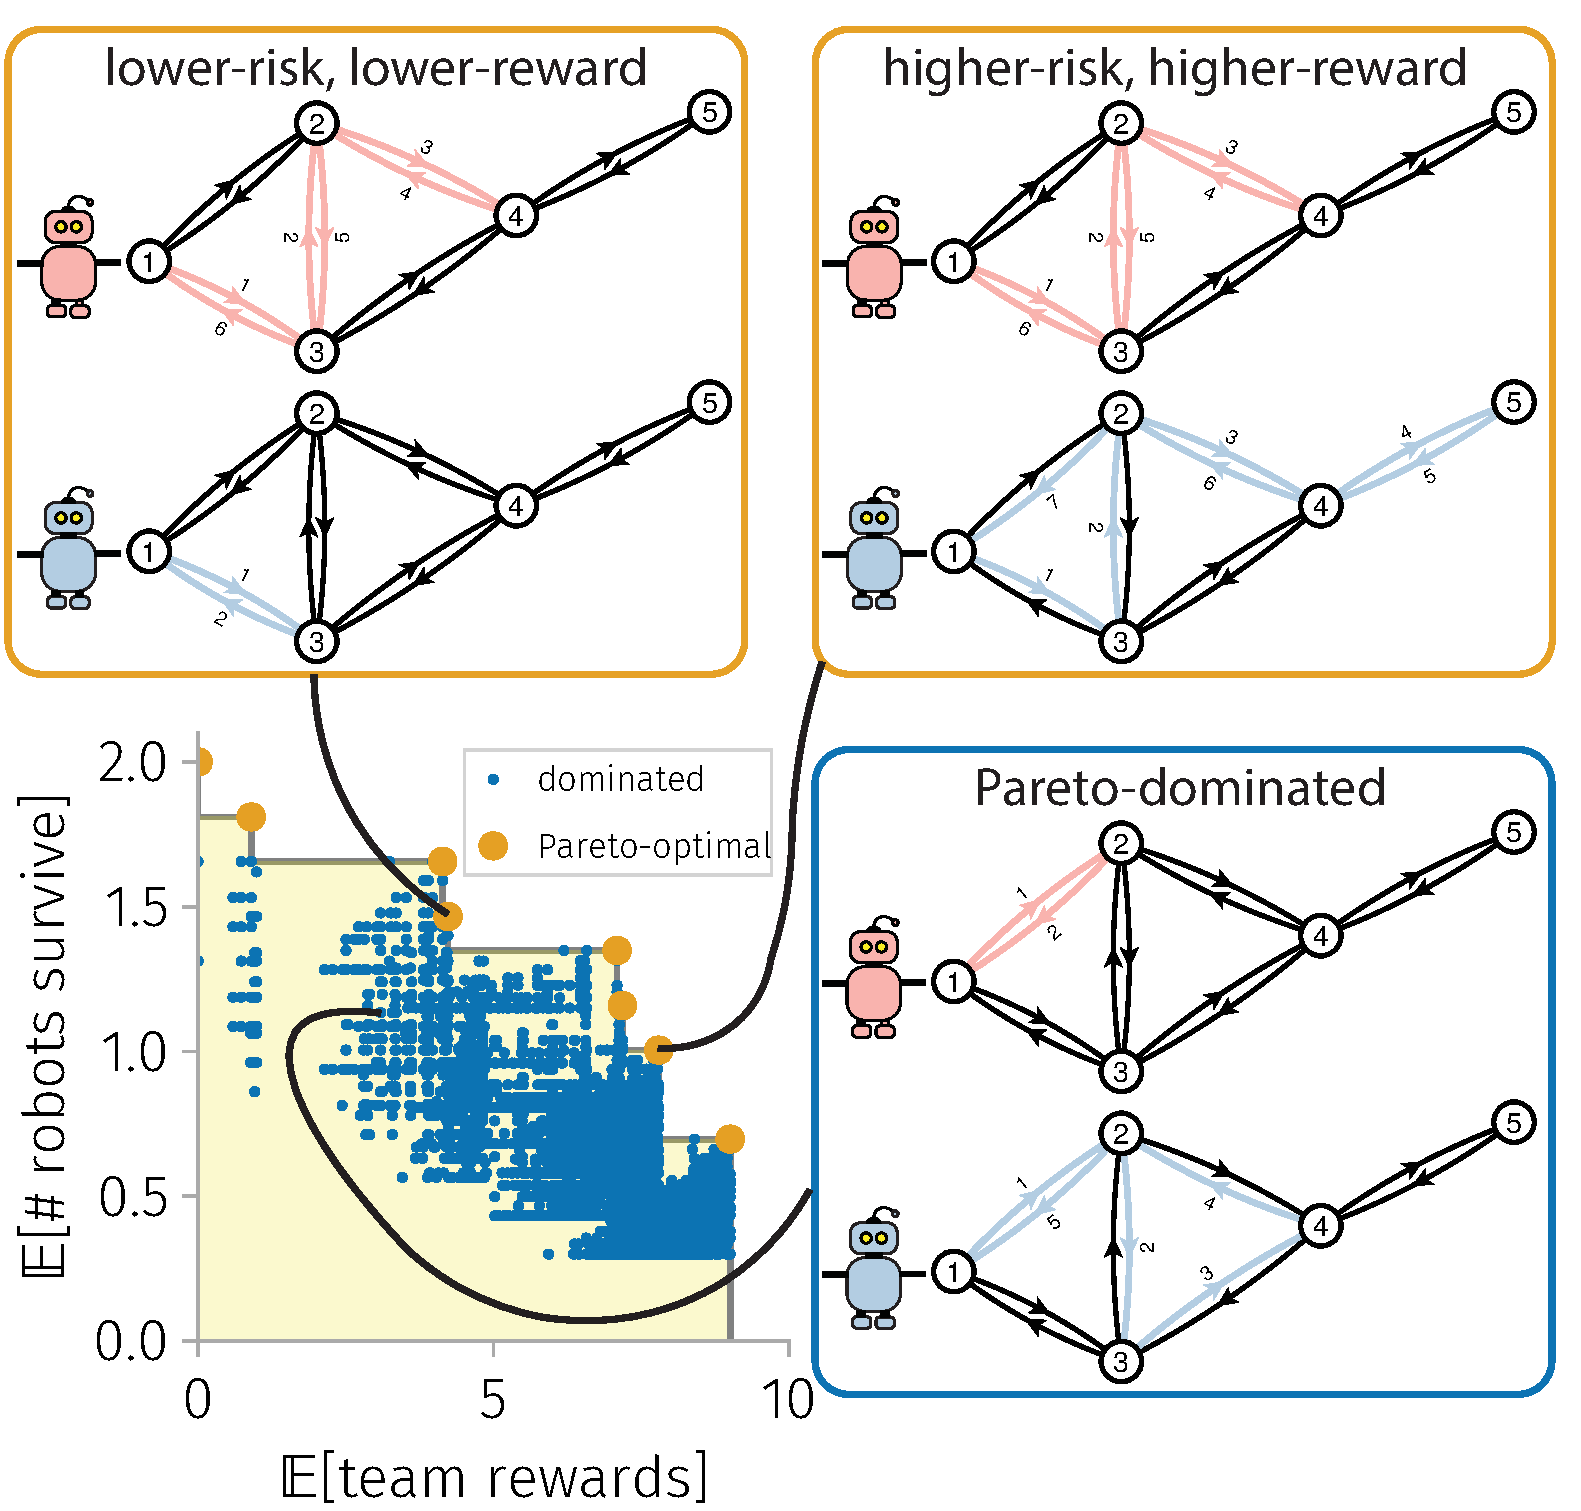
\includegraphics[width=\textwidth]{drawings/toy_pareto_front2.pdf}
	\caption{} \label{fig:pareto_optimal}
    \end{subfigure}
    \caption{
      The bi-objective team orienteering in hazardous environments problem (BOTOHE).
      (a) A team of robots are mobile on a directed graph whose 
      nodes offer a reward to the team if visited by a robot and 
      arcs present a probability of destruction to robots that traverse them (tornado = 1/10 probability of destruction). Our task is to plan the trails of the robots to maximize the expected reward collected and the expected number of robots that survive.
      (b) Pareto-optimal and -dominated robot-team trail plans scattered in objective space, with two Pareto-optimal plans and one Pareto-dominated plan shown.}
\end{figure}



\section{The bi-objective team orienteering in hazardous environments problem (BOTOHE)}
%In the risky team orienteering problem (RTOP), our task is to plan the trails of a team of mobile robots on a directed graph whose (i) nodes offer rewards to the team depending on the number of robots that visit them and (ii) edges, when traversed by a robot, impose a risk of robot failure/destruction.
%The trails are set at the beginning of the mission, then followed by the robots without updates during the mission---an offline setting. 
%For the bi-objective RTOP (BO-RTOP), we wish to find the set of Pareto-optimal trail plans for the robot team that maximize the expected (i) rewards collected by the team and (ii) the number of robots that survive the mission.




\subsection{Problem setup}
Here, we pose the bi-objective robot-team orienteering in hazardous environments problem (BOTOHE).

\paragraph{Spatial abstraction of the environment as a directed graph.}
We model the environment as a directed graph $G=(\mathcal{V}, \mathcal{E})$, where $\mathcal{V}$ is its set of vertices and $\mathcal{E}$ is its set of directed edges (=arcs =ordered pairs of distinct vertices). We assume $G$ is strongly connected, but not necessarily complete. We enforce one self-loop $(v_b, v_b) \in \mathcal{E}$ to allow the possibility for a robot to never leave the base node.

\vspace{-\baselineskip}
\subparagraph{Interpretation.} 
Each node $v\in \mathcal{V}$ represents a distinct location in the environment (e.g., a room in a building or a house in a neighborhood).
Each arc $(v, v^\prime) \in \mathcal{E}$ represents a direct spatial connection (e.g., a doorway or a road) for traveling from location $v$ to location $v^\prime$.


% the best (e.g., shortest or safest) path (in Euclidean space) for a mobile robot to take from the location represented by node $v$ to the location represented by $v^\prime$.
% Note, we do not assume the graph is complete\footnote{Ie., not every pair of distinct nodes $\{v, v^\prime\}$ is joined by two edges $(v, v^\prime)$ and $(v^\prime, v)$. 
% Eg., consider a building with node $v$ representing a room on the first floor, node $v^\prime$ a room on the second floor, and node $u$ as the staircase between the first and second floors. Traveling from node $v$ to node $v^\prime$ necessitates passing through node $u$ first.}.

\paragraph{The team of mobile robots.}
A homogenous team of $K$ robots all begin at a base station represented by node $v_b \in \mathcal{V}$ of the graph $G$. The robots are \emph{mobile} in the environment, meaning they may walk on the graph $G$.
Ie., each robot can sequentially hop from a node $v$ to another node $v^\prime$ via traversing arc $(v, v^\prime)\in\mathcal{E}$.

\paragraph{Team rewards offered by nodes in the graph.}
Each node $v\in \mathcal{V}$ in the graph $G$ offers a reward to the robot team if visited by a robot over the course of the mission.
The node reward map $r: \mathcal{V} \rightarrow \mathbb{R}$ quantifies the reward offered to the team by each node. 
% visits node $v$ receives by a robot over the course of the mission
The total reward collected by the team is additive among nodes of the graph.
 
Note, 
(1) even if a robot is destroyed after leaving node $v$, it still counts as a successful visit to node $v$ to extract its reward $r(v)$;
(2) multiple visits to a node do not provide further marginal reward over a single visit; and
(3) the reward offered by a node could be negative, ie. there could be a penalty to visit a node instead of an incentive.

\vspace{-\baselineskip}
\subparagraph{Interpretation.} The rewards given by a node represent the utility gained by the team when eg. a robot delivers a resource to the node, takes an image of the node and transmits it back to the command center, actuates some process (eg. turn a valve) at the node, etc. 


\paragraph{The probabilistic model of robot destruction during trail-following.} 
Each robot incurs a risk of destruction when it traverses an arc of the graph $G$.
% following its trail $\rho$. 
Specifically, starting (in a functioning state) at some node $v$, a robot survives with probability $\omega(v, v^\prime)$ the two-step process of (i) traversing arc $(v, v^\prime) \in \mathcal{E}$ then (ii) visiting node $v^\prime$. 
We assume (i) each outcome (survival or destruction) of this two-step process is an independent event and (ii) the survival probabilities are static over the course of the mission. 
Thus, from the function $\omega: \mathcal{E} \rightarrow (0, 1]$ that assigns robot survival probabilities to each arc of the graph $G$, we can compute the survival probabilities of the $K$ robots following any given set of trails.
% plans $\{\rho_1, ..., \rho_K\}$.% and (2) the expected utility of the rewards harvested by the robots along their paths, which we write next. 



\vspace{-\baselineskip}
\subparagraph{Interpretation.} The hazards in the environment could originate from obstacles the robot could crash into, rough terrain or seas, severe weather, mines, corrosive chemicals, or adversaries capable of attacking the robots at the arcs and/or nodes.
The stochasticity of the survival of a robot traversing an arc originates from eg. (i) the unpredictability of an aerial robot crashing into an obstacle, a ground robot falling over rocks, or a surface aquatic robot succumbing to ocean waves, or (ii) adversaries with (a) an imperfect capability to detect and attack robots and/or (b) uncertain presence in the environment.

\vspace{-\baselineskip}
\subparagraph{Possible asymmetry.} We do not assume $\omega$ is symmetric, ie., that $\omega(v, v^\prime) = \omega(v^\prime, v)$. The traversal from node $v$ to $v^\prime$ may be more dangerous than from $v^\prime$ to $v$ owing to eg., (i, asymmetric arc traversal) strong air or water currents in the direction $v^\prime$ to $v$ or (ii, asymmetric dangers at nodes) an adversary with attack capability at node $v^\prime$ but not at $v$. %Even if edge traversal risks are symmetric, the action of visiting a node be risky, and node $v$ may be more or less dangerous than node $v^\prime$, breaking symmetry. 

\paragraph{The robot-team trail plan.}
To collect rewards, robot $k$ on the team will plan to execute/follow a closed, directed trail $\rho_k$ on the graph $G$.  
The set\footnote{Since the robot team is homogenous, we consider the optimal trail plans for the robots as permutation-invariant and thus track it as a set not a list.} of closed, directed trails $\mathcal{P}:=\{\rho_1, ..., \rho_K\}$ the robot-team plans to follow constitute the \emph{robot-team trail plan} for the \emph{mission}. 
This constitutes only a ``plan'' because a robot may be destroyed in the process of following its planned trail and thus not actually visit all nodes in its trail plan.

\vspace{-\baselineskip}
\subparagraph{A closed, directed trail.} 
A \emph{directed trail} is an ordered list of nodes $\rho = (\rho[0], \rho[1], ..., \rho[\lvert \rho \rvert])$ where
(i) $\rho[i] \in \mathcal{V}$ is the $i$th node in the trail,  
(ii) an arc exists from each node in $\rho$ to the subsequent node, ie., $(\rho[i-1], \rho[i])\in\mathcal{E}$ for $1 \leq i  \leq \lvert \rho \rvert$,
(iii) $\lvert \rho \rvert$ is the number of arcs traversed in the trail,
and
(iv) the arcs traversed in the trail are unique, ie. each arc in the multiset $\{(\rho[i-1], \rho[i])\}_{i=1}^{\lvert \rho \rvert}$ has a multiplicity of one.
Note, unlike a path, the nodes in a trail are not necessarily distinct \cite{wilson1979introduction}.
A \emph{closed} trail begins and ends at the same node, ie. $\rho [0]=\rho[\lvert \rho \rvert]$, which, here, $=v_b$.

\vspace{-\baselineskip}
\subparagraph{The static/offline setting.} 
The robot-team trail plan $\mathcal{P}$ are set at the beginning of the mission, then followed by the robots without adaptation or updates during the mission in response to observing robot failure(s).
Ie., robots cannot communicate their survival status to the command center during the mission and/or the command center cannot send updated instructions to the robots after the mission executes.

\paragraph{The two objectives.}
The total team \underline{r}ewards collected by the robot-team, $R$, and the number of robots that ultimately \underline{s}urvive the mission, $S$, both (i) depend on the robot-team trail plan $\mathcal{P}$ and (ii) are random variables owing to the stochasticity of robot survival while trail-following.
Given 
the directed graph $G$ as a spatial abstraction of the environment, 
the homogenous team of $K$ mobile robots starting at the base node $v_b$,
the node reward functions $\{r_v : v \in\mathcal{V}\}$, 
and the arc survival probability map $\omega$, 
the BOTOHE problem is to determine the optimal robot-team [closed] trail plan $\mathcal{P}$ that maximizes two-objectives, (1) the expected team-reward and (2) the expected number of robots that survive the mission:
\begin{equation}
\max_{\mathcal{P}=\{\rho_1, ..., \rho_K\}} \left( \mathbb{E}[R(\mathcal{P})], \mathbb{E}[S(\mathcal{P})] \right).
\label{eq:the_two_objs}
\end{equation}

%\vspace{-\baselineskip}
%\subparagraph{Objective \#1: the expected reward collected by the robots.}
%Let $T_v(\mathcal{P}) $ be the number of robots on the team with trail plans $\mathcal{P}$ that ultimately visit node $v$.
%Because of the stochasticity of robot survival while trail-following, and thus of which nodes in the trail plan each robots ultimately visits, $T_v$ is a random variable.
%Then, the total team \underline{r}ewards collected by the robot-team following trail plans $\mathcal{P}$ is also a random variable:
%\begin{equation}
%R(\mathcal{P}) = \sum_{v\in\mathcal{V}} r_v\left ( T_v(\mathcal{P}) \right)
%\end{equation}
%that sums the rewards received from each node of the graph $G$.
%
%\vspace{-\baselineskip}
%\subparagraph{Objective \#2: the expected number of robots that survive the mission.}
%Let $S(\mathcal{P})$ be the number of robots, on a robot team with trail plans $\mathcal{P}$, that ultimately \underline{s}urvive the mission. Because of the stochasticity of robot survival while trail-following, $S$ is a random variable. 
%
%We wish to devise robot-team trail plans $\mathcal{P}$ to maximize both (1) the expected team reward, $\mathbb{E}[R(\mathcal{P})]]$, and (2) the expected number of robots that survive the mission, $\mathbb{E}[S(\mathcal{P})] \in (0, K]$. We derive formulas for the values of the two objectives in terms of the robot-team trail plans later (see eqns.~\ref{eq:formula_obj1} and \ref{eq:formula_obj2}). 


\subparagraph{Comparison with TSOP.}
The BOTOHE formulation follows the TSOP \cite{jorgensen2018team} with four modifications: we (i) omit the constraints that each robot survives above a threshold probability\footnote{Ie., we accept if one [unmanned] robot bears much more risk of destruction than another during the mission.}, (ii) allow robots to follow trails instead of restricting to paths, as paths prevent robots from visiting a given node more than once and thus from e.g., harvesting reward from a node with an in- and out-degree of one, (iii) aim to maximize two objectives instead of one, and (iv) do not assume the team reward viewed as a function over the set of visited nodes is monotone because we allow for negative rewards.
{\color{red} k then make this happen in example, and how then does $\eta_r$ work if it can be negative? }

\paragraph{Seeking the Pareto-optimal set of robot-team trail plans.} 
In most problem instances, the bi-objective problem in eqn.~\ref{eq:the_two_objs} presents a conflict between designing the robot-team trail plan to maximize the expected reward vs. the expected number of surviving robots. Ie., a utopian robot-team trail plan that simultaneously maximizes \emph{both} objectives is unlikely to exist.
Focusing solely on the survival objective, the robots safely stay at the base station and do not attempt to collect any rewards---no matter the [positive] size of the rewards to be gained by leaving the base station. 
Focusing solely on the reward objective, each robot plans to visit every node offering a positive reward---no matter the risk to survival involved. Such node-visitation redundancy endows the team reward with robustness to robot failures.

Given the conflict between the two objectives, the ultimate robot-team trail plan selected for the mission must make a tradeoff between the expected reward and the expected number of robots that survive. 
A human decision-maker must invoke their values to make this tradeoff.
Valuing survival more than rewards will favor trail-plans where robots do not enter dangerous regions of the environment, even if large rewards are offered there. 
Valuing rewards more than survival will instead send robots into these dangerous regions to attempt collection of those rewards. 

Herein, solving the bi-objective optimization problem in eqn.~\ref{eq:the_two_objs} constitutes finding the Pareto-optimal set of team-robot trail plans. Then, we can present the Pareto set to the decision-maker, who ultimately selects the team-robot trail-plan according to their values placed on team-reward vs. robot survival. 

\subparagraph{Pareto-optimal team-robot trail plans.} 
A \emph{Pareto-optimal} \cite{pardalos2017non} robot-team trail plan $\mathcal{P}^*$ cannot be altered to
(1) increase the survival objective $\mathbb{E}[S]$ without compromising (decreasing) the reward objective $\mathbb{E}[R]$
nor
(2) increase the reward objective $\mathbb{E}[R]$ without compromising (decreasing) the survival objective $\mathbb{E}[S]$.
Formally, plan $\mathcal{P}^*$ belongs to the Pareto-optimal set of plans if no other plan $\mathcal{P}^\prime$ \emph{Pareto-dominates} it. By definition, a plan $\mathcal{P}^\prime$ Pareto-dominates plan $\mathcal{P}^*$ if:
\begin{align}
	\left (\mathbb{E}[R(\mathcal{P}^\prime)] \geq \mathbb{E}[R(\mathcal{P}^*)]  \right) & \wedge \left( \mathbb{E}[S(\mathcal{P}^\prime)] \geq \mathbb{E}[S(\mathcal{P}^*)] \right) \\
	\left( \mathbb{E}[R(\mathcal{P}^\prime)] > \mathbb{E}[R(\mathcal{P}^*)] \right) & \vee \left( \mathbb{E}[S(\mathcal{P}^\prime)] > \mathbb{E}[S(\mathcal{P}^*)] \right).
\end{align}
Clearly, if a plan $\mathcal{P}^\prime$ were to Pareto-dominate another plan $\mathcal{P}^*$, one would never choose plan $\mathcal{P}^*$ over plan $\mathcal{P}^\prime$, regardless of how we relatively value the two objectives. The \emph{Pareto front} is the set of objective vectors $\{(\mathbb{E}[R], \mathbb{E}[S])\}$ associated with the Pareto-optimal set of robot team trail plans $\{\mathcal{P}^*\}$. See Fig.~\ref{fig:pareto_optimal}. 

\subsection{Probability distributions and expectations of $R(\mathcal{P})$ and $S(\mathcal{P})$}
We now derive formulas for the probability distributions and expectations of the team reward $R(\mathcal{P})$ and number of robots that survive the mission $S(\mathcal{P})$, depending on the robot-team trail plan $\mathcal{P}$. 
These formulas follow from the directed graph $G$, edge survival probability map $\omega$, and node reward map $r$. Fig.~\ref{fig:notation} illustrates our notation.

\begin{figure}[h!]
    \centering
    	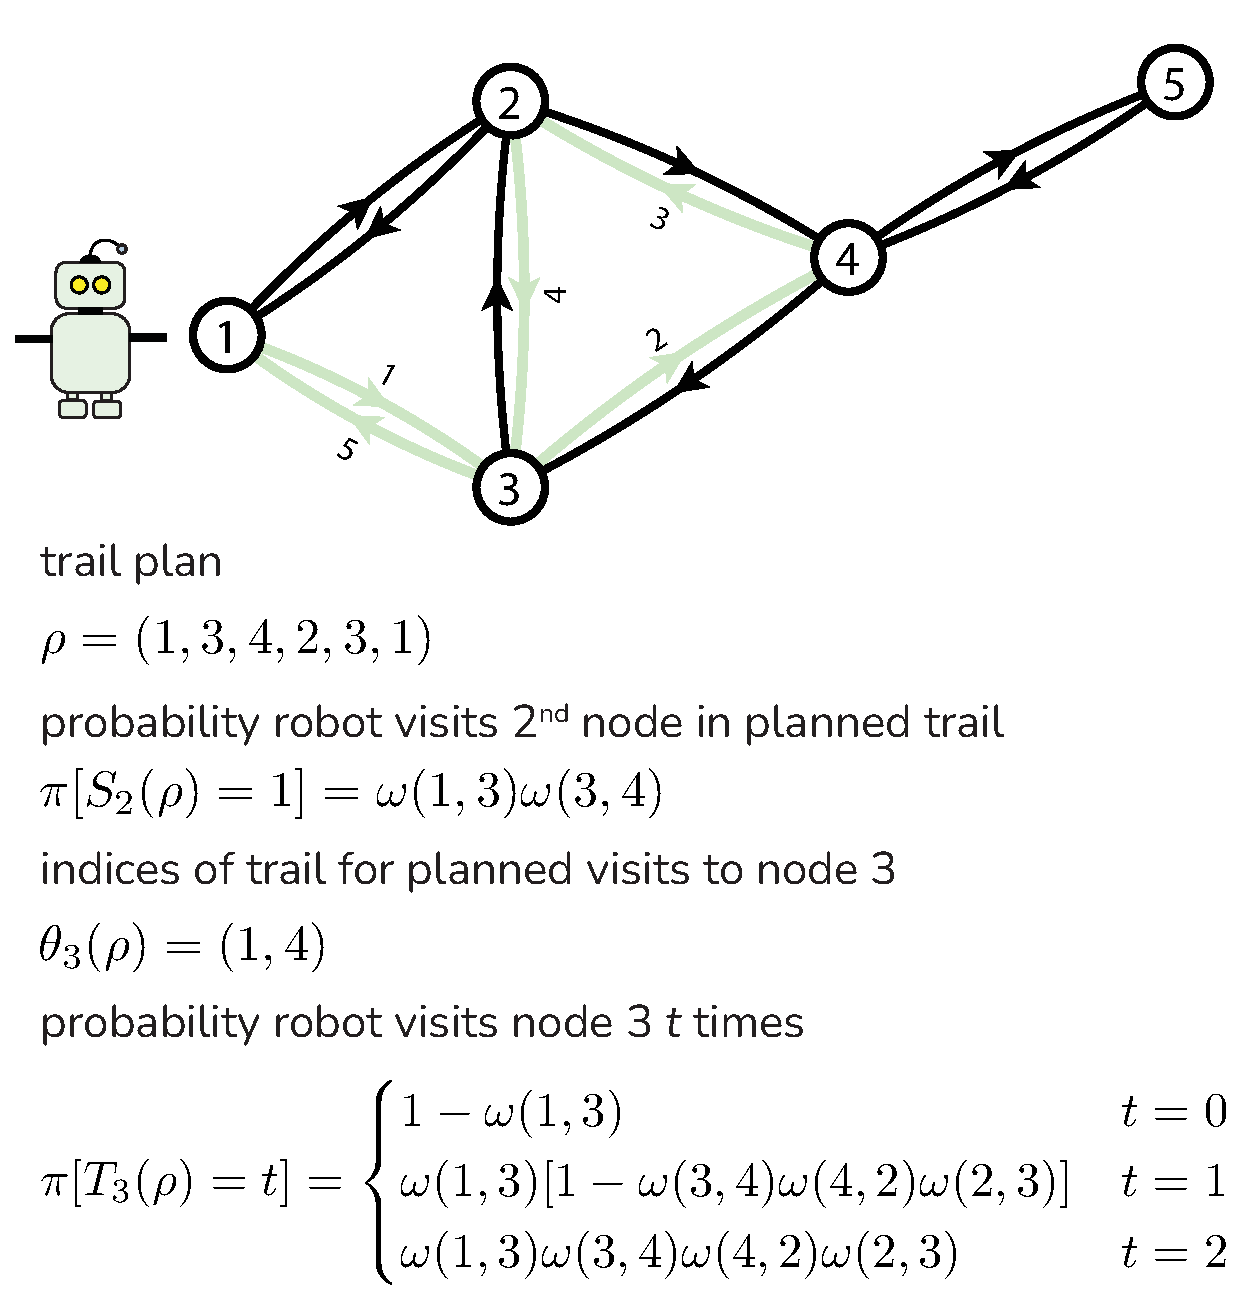
\includegraphics[width=0.6\textwidth]{drawings/notation_fig/notation.pdf}
    \caption{Illustrating notation for a particular robot trail plan.} \label{fig:notation}
\end{figure}

\paragraph{The survival of a single robot along its followed trail.} First, we write a formula for the probability that a robot survives to reach a given node in its planned trail.
For $0 \leq n \leq \lvert \rho \rvert$, 
Let $S_n(\rho)$ be the Bernoulli random variable that is one if a robot following trail $\rho$ survives to visit the $n$th node in the trail and zero otherwise. For the event of survival, the robot must survive traversal of \emph{all} of the first $n$ arcs in its trail to visit node $\rho[n]$. So, since the arc-traversal$+$node-visit survival events are independent, the probability that a robot following trail $\rho$ successfully visits node $\rho[n]$ is the product of the survival probabilities of the first $n$ arc-hops in the trail:
\begin{align}
	\pi[S_n(\rho) = 1] & = \prod_{i=1}^n \omega(\rho[i-1], \rho[i]) \label{eq:pi_S_n} \text{ for } 0 \leq n \leq \lvert \rho \rvert \\%\in \{1, ..., \lvert \rho \rvert\} 
	& = 1 - \pi[S_n(\rho) = 0]. \label{eq:pi_S_n_0} 
\end{align} %The factorization owes to the independence of the arc-traversal$+$node-visit survival events.
The second line follows because the complement of the event of survival is destruction.

Note, the outcome $S_n(\rho)=0$ implies $S_{n+i}(\rho)=0$ for $1 \leq i \leq \lvert \rho \rvert-n$ since, once a robot is destroyed at some node/arc along its trail, it cannot visit subsequent nodes in the planned trail.

\paragraph{The number of robots on the team that survive the mission.} 
Now, we write a formula for the second objective, the expected number of robots that survive the mission, $\mathbb{E}[S(\mathcal{P})]$.
The event of survival of each robot is independent of the other robots.
Consequently, the number of robots that survive the mission, $S$, is the sum of the Bernoulli random variables indicating the survival of each robot over its planned trail:
\begin{equation}
	S(\mathcal{P}=\{\rho_1, ..., \rho_K\})=\sum_{k=1}^K S_{\lvert \rho_k \rvert}(\rho_k). \label{eq:R_sum}
\end{equation}
Thus, $S$ follows the Poisson-Binomial distribution \cite{tang2023poisson}.
Specifically, the probability that $s$ robots survive the mission is:
\begin{multline}
	\pi[S(\mathcal{P})=s] = \sum_{\substack{\mathcal{R} \subseteq \{1, ..., K\}  \\ \lvert \mathcal{R} \rvert = s} } \,
	\prod_{k \in \mathcal{R}} \pi[S_{\lvert \rho_k \rvert}(\rho_k) = 1]
	\prod_{k^\prime \in \{1, ..., K\} \setminus \mathcal{R}}
	 \pi[S_{\lvert \rho_{k^\prime} \rvert}(\rho_{k^\prime}) = 0]
	 , \\ \text{ for } 0 \leq s \leq K.
	\label{eq:R_pb}
\end{multline}
Eqn.~\ref{eq:R_pb} sums over all $\binom{K}{s}$ possible size-$s$ surviving subsets $\mathcal{R}$ of the $K$ robots. The first product is the probability that all of those robots in $\mathcal{R}$ indeed survive their closed trails. The second product is the probability that the other robots outside of $\mathcal{R}$ indeed get destroyed somewhere along their closed trails.
Seen from eqn.~\ref{eq:R_sum} and the linearity of the expectation operator, the expected number of robots that survive the mission is:
\begin{equation}
	\mathbb{E}[S(\mathcal{P}=\{\rho_1, ..., \rho_K\})]=\sum_{k=1}^K \mathbb{E}[S_{\lvert \rho_k \rvert}(\rho_k)] = \sum_{k=1}^K  \pi[S_{\lvert \rho_k \rvert}(\rho_k) = 1] \label{eq:formula_obj2}
\end{equation} with $\pi[S_{\lvert \rho_k \rvert}(\rho_k) = 1]$ given in eqn.~\ref{eq:pi_S_n}.

\paragraph{The probability a given node is not visited by a single robot.} 
To calculate the expected team reward, we first calculate the probability that a robot following a given trail does not visit a given node.
Let the Boolean random variable $T_v(\rho)$ be one if robot following trail $\rho$ visits node $v\in \mathcal{V}$ and zero if it does not.
If node $v$ is not in the planned trail $\rho$, $T_v(\rho)=0$ with certainty. 
Now, suppose node $v$ is in the planned trail $\rho$. Let $n^*$ be the index in the trail where the robot plans its first visit to node $v$:
\begin{equation}
n^*(\rho, v) = \min_{
	\substack{n \in \{0, ..., \lvert \rho \rvert\} \\ \rho[n] = v}
} n.
\end{equation}
Then, $T_v(\rho)$ is equal to the random variable $S_{n^*}(\rho)$ because the robot must survive its first $n^*$ arc-hops to successfully visit node $v$. 
So, the probability node $v$ is not visited by a robot following trail $\rho$ is:
\begin{equation}
	\pi[T_v(\rho) = 0] = 
	\begin{cases}
		1 & v\notin \rho\\
		 \pi [S_{n^*(\rho, v)}(\rho)=0 ] & v \in \rho
	\end{cases}
	 \label{eq:pi_T_v}
\end{equation}
with $\pi[S_{n^*}(\rho)=0]$ calculated using eqn.~\ref{eq:pi_S_n_0}.

\paragraph{The probability a given node is visited by one or more robots on the team.} 
Now, let $T_v(\mathcal{P}=\{\rho_1, ..., \rho_K\} )$ be the Boolean random variable that is one if one or more robots on the team with trail plans $\mathcal{P}$ visit node $v$ and zero otherwise.
The latter occurs if and only if zero of the robots visit node $v$. Hence,
\begin{equation}
	\pi [T_v(\{\rho_1, ..., \rho_K\} ) = 1)] = 
	1 - \prod_{k=1}^K \pi[T_v(\rho_k)=0].
	\label{eq:pi_T_v_all}
\end{equation} 
with $\pi[T_v(\rho) = 0]$ in eqn.~\ref{eq:pi_T_v}.

\paragraph{The expected team reward.}
Finally, the total team reward collected by the robot-team following trail plan $\{\rho_1, ..., \rho_K\}$ is the sum of the rewards given to the team by each node:
\begin{equation}
R(\{\rho_1,...,\rho_K\}) = \sum_{v\in\mathcal{V}} r(v)  T_v(\{\rho_1, ..., \rho_K\}),
\end{equation} where the reward from node $v$, $r(v)$, is collected if and only if node $v$ is visited by one or more robots (i.e. iff $T_v(\mathcal{P})=1$).
Finally, the expected reward accumulated over the mission by a robot-team following trail plans $\{\rho_1, ..., \rho_K\}$ is:
\begin{equation}
	\mathbb{E}[R(\{\rho_1,...,\rho_K\})]= \sum_{v\in\mathcal{V}} r(v) \pi[T_v(\{\rho_1, ..., \rho_K\}) = 1] \label{eq:formula_obj1}
\end{equation}
with $ \pi[T_v(\{\rho_1, ..., \rho_K\}) = 1]$ given in eqn.~\ref{eq:pi_T_v_all}.

\paragraph{Summary.} Given a proposed robot-team trail plan $\mathcal{P}$, we can calculate the two objectives $\mathcal{E}[R(\mathcal{P})]$ and $\mathcal{E}[S(\mathcal{P})]$ via eqns.~\ref{eq:formula_obj1} and \ref{eq:formula_obj2}, respectively.
% harvest risk different from visit risk. once harvested, then no longer risk for other robots to visit that node.

\section{Bi-objective ant colony optimization to search for the Pareto-optimal robot-team trail plans}
To efficiently search for the Pareto-optimal set of robot-team trail plans defined by eqn.~\ref{eq:the_two_objs}, we employ bi-objective (BO) ant colony optimization (ACO) \cite{iredi2001bi}. 

ACO \cite{dorigo2006ant,bonabeau1999swarm,blum2005ant} is a meta-heuristic for combinatorial optimization problems framed as a search for an optimal path (or trail) through a graph.
As a swarm intelligence method \cite{bonabeau1999swarm}, ACO is inspired by\footnote{
Though ACO is heavily inspired by ants laying and following pheromone trails during foraging, an important point is that ACO is intended and designed to be a useful system for solving optimization problems---not as a model that faithfully replicates the foraging behavior of ants. 
Consequently, ACO lacks many features of real ants foraging for food and does not adhere to biologically plausible parameters for e.g. pheromone deposition and evaporation. \cite{bonabeau1999swarm}
}
 the behavior of ants foraging for food \cite{bonabeau2000inspiration}. See Box~\ref{box:ants}. 
Variants of the single-robot- and team- orienteering problem have been efficiently and effectively solved by ACO \cite{ke2008ants,chen2015multiobjective,verbeeck2017time,sohrabi2021acs,chen2022environment}\footnote{Other [meta-]heuristics have been applied to the orienteering problem as well \cite{gavalas2014survey,dang2013effective,chao1996fast,butt1994heuristic}.}.

\begin{mybox}[label=box:ants, breakable]{Ants lay and follow pheromone trails to collectively select the shortest trail to the highest-quality food source}
When a member of an ant colony discovers a highly-quality food source, it is advantageous to mobilize the colony to exploit this food source \cite{deneubourg1983probabilistic} and to take the \emph{shortest} path between the nest and the food \cite{goss1989self}.

Some species of foraging ant colonies can collectively, when presented with
(i) two equi-distant food sources of differing quality, select the highest-quality food source \cite{beckers1993modulation} and
(ii) two paths between the nest and a food source, select the shortest path \cite{goss1989self}.
% Now, ants, as individuals, possess limited intelligence \cite{edelstein1995trail}.
Remarkably, the ants achieve this, despite possessing limited intelligence \cite{edelstein1995trail}, largely [though not exclusively \cite{evison2008combined,czaczkes2015trail,robinson2005no}] via a mechanism excluding central control, \emph{direct} communication with each other, individual memory, and a global [conceptual or visual] view of the environment: by laying and following pheromone trails \cite{czaczkes2015trail}.

As worker ants travel from a food source back to the nest, they deposit pheromone, a relatively volatile chemical substance \cite{david2009trail}, on the ground. 
This pheromone marks trails to food sources and, as an olfactory cue \cite{knaden2016sensory}, signals to other ants in the colony to follow it. \cite{david2009trail,deneubourg1990self}
Ants tend to both 
(i) modulate the amount of pheromone they deposit based on the quality of the food source \cite{beckers1993modulation}
and
(ii) follow pheromone trails with higher concentrations of pheromone \cite{beckers1993modulation,czaczkes2015trail}. 
% The amount of pheromone they deposit is modulated by the quality of the food source . 
This explains how an ant colony can collectively select the highest quality food source when presented with multiple equidistant options. 
As for finding shortest paths, consider an ensemble of ants initially exploring multiple paths from a high-quality food source back to the nest.
The ants taking the shorter paths return to the nest and complete their pheromone trails sooner. These shorter trails, compared to longer trails, then most quickly recruit new ants, accumulate pheromone, and get reinforced. By this positive feedback mechanism, ants are mass-recruited to take the shortest path from the nest to a food source. \cite{jackson2006communication,czaczkes2015trail,bonabeau1999swarm}

Negative feedback mechanisms are present as well. 
First, pheromone also evaporates over time \cite{jackson2006communication}.
When a food source is exhausted, the ants no longer lay pheromone on the way back to the nest. The concentration of pheromone on this trail then decays over time due to evaporation \cite{david2009trail,van2011temperature}. Advantageously, then, ants are not [wastefully] recruited to that location anymore. 
Second, ants deposit less pheromone on trails that (i) already have high pheromone concentrations \cite{czaczkes2013ant} or (ii) lead to food sources already occupied by their nestmates \cite{wendt2020negative}.

Importantly, all ants do not deterministically select the trail with the highest pheromone concentration, without ``error'' \cite{deneubourg1990self}.
To a degree, this stochasticity in the process of ants choosing a trail is beneficial for 
(i) exploration in the explore-exploit tradeoff during foraging, 
(ii) exploiting multiple food sources in parallel, 
and 
(iii) endowing the colony with plasticity in a dynamic environment (e.g. introduction of new, higher-quality food sources) \cite{deneubourg1983probabilistic,shiraishi2019diverse,deneubourg1986random,dussutour2009noise,edelstein1995trail}.

Finally, some ants can deposit multiple species of pheromone (from different glands) with eg. different longevities \cite{czaczkes2015trail}, allowing for more complex indirect communication \cite{jackson2006communication} eg. a ``no entry'' signal \cite{robinson2005no}. 

In summary, pheromone trails of an ant colony abstractly constitute a collective memory, a local guide for ants to high-quality food sources and short paths to them, and a medium through which ants indirectly communicate \cite{jackson2006communication}. 
The positive feedback, negative feedback, and randomness in the behavior of many decentralized agents like ants laying and following pheromone trails enables self-organization of the colony \cite{bonabeau1997self}, where ``complex collective behaviors may emerge from interactions among individuals that exhibit simple behaviors''.
Simple models of ants laying and probabilistically following pheromone trails (some with evaporation) indeed reproduce salient features of ants foraging \cite{bonabeau1999swarm,goss1989self,jackson2006communication,edelstein1995trail,watmough1995modelling}.
\end{mybox}

We describe the bi-objective ACO \cite{iredi2001bi} algorithm we employ to find the Pareto-optimal robot-team trail plans defined by eqn.~\ref{eq:the_two_objs}. 

Bi-objective ACO proceeds iteratively. 
At each iteration, each artificial ant in the heterogeneous colony constructs a robot-team trail plan $\{\rho_1, ..., \rho_K\}$---robot by robot, arc by arc.
The ant constructs trails stochastically, guided by (i) two species of pheromone on the arcs, one for the reward objective, one for the survivability objective, and (ii) greedy heuristics that score the myopic desirability of taking each arc. 
At the end of each iteration, the ants compare the robot-team trail plans they constructed. 
Ants that found Pareto-optimal robot team trail plans, both over plans (i) in that iteration only and (ii) over all past iterations, deposit pheromone (of each species) on each arc belonging to these trails. The amount of pheromone an ant deposits is proportional to the value of the objective (associated with that species) achieved under the plan that ant found.
To prevent stagnation and promote continual exploration, the pheromone evaporates each iteration as well.
The ants communicate the trails they found with an elitist ant who maintains a set of, over all team trail plans constructed by all ants over all iterations, the Pareto-optimal robot-team trail plans. 
The algorithm terminates after a pre-specified number of iterations and returns the Pareto-optimal robot-team trail plans maintained by the elitist ant. 
Note, as ACO is a meta-heuristic, it is not guaranteed to find all Pareto-optimal solutions nor neglect to include a Pareto-dominated solution. I.e., the ACO algorithm returns an \emph{approximate} Pareto-optimal set of robot-team trail plans.
%A colony of artificial ants collaborate in their search for Pareto-optimal team trail plans. At 
%ACO is an iterative algorithm. 

\paragraph{A heterogeneous colony of artificial ants.}
We create a colony of $N_{\text{ants}}$ artificial ants.
Every iteration, each ant searches for a Pareto-optimal robot-team trail plan $\{\rho_1, ..., \rho_K\}$.
To dictate how an ant balances the two objectives during its search, it is assigned a parameter $\lambda \in [0, 1]$, where $\lambda$ closer to zero (one) implies the ant prioritizes maximizing the expected reward $\mathbb{E}[R]$ (expected robot survivals $\mathbb{E}[S]$). 
Particularly, ant $i\in\{1, ..., N_{\text{ants}}\}$ in the colony is assigned $\lambda_i := (i-1) / (N_{\text{ants}}-1)$.
This heterogeneity in the colony provides some division of labor in the colony: different ants focus on finding trail-plans in different regions of the Pareto front. 

\paragraph{An elitist ant.} In addition, the colony communicates the trail-plans they found to an elitist ant \cite{dorigo1996ant} that maintains a memory of the Pareto-optimal team-robot trail plans found over \emph{all} previous iterations. The elitist ant does not build a team trail plan of its own.


\paragraph{Pheromone on the arcs of the graph $G$.}
The ants lay and [probabilistically] follow two distinct species of artificial pheromone on the arcs of the graph $G$---one species associated with each objective. 
The pheromone maps $\tau_R:\mathcal{E}\rightarrow \mathbb{R}_+$ and $\tau_S:\mathcal{E}\rightarrow \mathbb{R}_+$ give the amount of reward and survivability pheromone, respectively, on each arc of $G$.
E.g., the amount of reward pheromone on arc $(v, v^\prime)\in\mathcal{E}$, $\tau_R(v, v^\prime)$, scores the promise of that arc, learned from all past experience of the ants, for belonging to robot trails that maximize the expected reward $\mathbb{E}[R]$. A similar interpretation holds for $\tau_S(v, v^\prime)$. 
Note, the pheromone maps are not static, but change from iteration-to-iteration due to both deposition by the ants and evaporation. 
Together, the pheromone maps constitute a collective, but fading, memory of the artificial ant colony---a memory of the propensity of each arc to belong to Pareto-optimal robot-team trail plans and, vaguely, where along the Pareto-front those plans might lie.
% vaguely, through laying and following \emph{two} species of pheromone, .

 
\paragraph{Robot-team trail-building by an ant.}
Each iteration, every ant in the colony constructs a robot-team trail plan $\{\rho_1, ..., \rho_K\}$.
The ant sequentially allocates trails to the robots, 
% It assigns trails to the robots sequentially, robot-by-robot. 
i.e. fully constructs the closed trail for robot 1, $\rho_1$, then $\rho_2$ for robot 2, and so on, up to robot $K$.
For each trail it constructs, the ant starts at the base node $v_b$, then, arc-hop by arc-hop, constructs the closed trail on the graph that the robot will follow. 

Trail construction is a stochastic process. Suppose the ant with objective-balancing parameter $\lambda$ is constructing the closed trail for robot $k$, $\rho_k$, and currently resides at node $v=\rho_k[i]$.
I.e., the ant has chosen the first $i$ arc-hops of robot $k$'s trail, with the partial trail being $\tilde{\rho_k}=(v_b, \rho_k[1], ..., \rho_k[i]=v)$.
The partial-trail extension rule gives the probability of next hopping to node $v^\prime\in\mathcal{V}$; it is the probability mass function $\pi[v^\prime \mid \rho_1, ..., \rho_{k-1}, \tilde{\rho}_k]$ over all nodes $v^\prime \in \mathcal{V}$ for extending the partial trail i.e.\ for setting $\rho_k[i+1]:=v^\prime$.
% termination criteria

\subparagraph{Feasible next-nodes in the trail.}
For node $v^\prime$ to be a candidate as the next node in the trail $\rho_k[i+1]$, arc $(v, v^\prime)$ must exist and (by definition of a trail) this arc mustn't have already been traversed in the partial trail $\tilde{\rho_k}$. 
So, the feasible set of next-nodes in the trail are:
%\begin{equation}
% 	\mathcal{V}^\prime := \{ v^\prime : (v, v^\prime ) \in \mathcal{E} \land \nexists j \in \{0, ..., i-1\} : (\tilde{\rho_k}[j], \tilde{\rho_k}[j+1])= (v, v^\prime)  \}.
%\end{equation}
\begin{equation}
 	\mathcal{V}^\prime := \{ v^\prime : (v, v^\prime ) \in \mathcal{E} \setminus \{ (\tilde{\rho_k}[j], \tilde{\rho_k}[j+1]) : j \in \{0,...,i-1\} \}\}.
\end{equation}
% Finally, if the current node is the base node ($v=v_b$), we augment the candidate set with $v_b$ ($\mathcal{V}^\prime \leftarrow \mathcal{V}^\prime \cup \{v_b\}$) to allow the closed partial trail to terminate, i.e. $\rho_k:=\tilde{\rho_k}$. Conceptually, this is equivalent to adding a self-loop $(v_b, v_b)$ to the set of arcs. This also allows a robot to never leave the base node.

 %(i, $\lvert \tilde{\rho_k} \rvert=1$) the robot to never leave the base node or (ii, $\lvert \tilde{\rho_k} \rvert >1$) the closed partial trail to terminate i.e. $\rho_k:=\tilde{\rho_k}$. 

\subparagraph{The partial-trail extension rule.}
% The ant selects the next node $\rho_k[i+1]=v^\prime$ in the trail $\rho_k$ from the candidate set $\mathcal{V}^\prime$ stochastically. 
The probability of choosing $\rho_k[i+1]:=v^\prime \in  \mathcal{V}^\prime$ depends on (i) the amount of each species of pheromone on arc $(v, v^\prime)$ that encodes ants' past experiences, (ii) the heuristic, experience-independent values $\eta_r(v, v^\prime)$ and $\eta_s(v, v^\prime)$ that score the [greedy] appeal, in terms of maximizing $\mathbb{E}[R]$ and $\mathbb{E}[S]$, respectively, of hopping from $v$ to $v^\prime$, and (ii) the objective-balancing parameter $\lambda$. Specifically,
\begin{multline}
	\pi(v^\prime \mid \rho_1, ..., \rho_{k-1}, \tilde{\rho_k}) \propto \\
		\begin{cases}
		 \left[\tau_R(v, v^\prime) \eta_r(v, v^\prime; \rho_1, ..., \rho_{k-1},\tilde{\rho_k}) \right]^{1-\lambda} \left[ \tau_S(v, v^\prime) \eta_s(v, v^\prime) \right]^\lambda & v^\prime \in \mathcal{V}^\prime (\tilde{\rho_k}) \\
		 0 & v^\prime \notin \mathcal{V}^\prime (\tilde{\rho_k}), \\
		 \end{cases}
	 \label{eq:prob_x_y}
\end{multline}
where we emphasize the dependence of $\eta_r$ on the ant's previously-constructed robot trails and the partial trail and of $\mathcal{V}^\prime$ on the partial trail.
Eqn.~\ref{eq:prob_x_y} makes ants more likely to traverse arcs with more pheromone and/or heuristic appeal, with more emphasis on the reward or survivability pheromone/heuristic depending on the ant's $\lambda$. Since the pheromone maps $\tau_{r,s}$ change from iteration-to-iteration, the transition rule in eqn.~\ref{eq:prob_x_y} also changes from iteration-to-iteration, as ants are hopefully biased towards arcs learned to be more promising based on past colony-level experience.

\subparagraph{Heuristics.} We now define the heuristic maps $\eta_s: \mathcal{E} \rightarrow \mathbb{R}_+$ and $\eta_r:  \mathcal{E} \rightarrow \mathbb{R}_+$ that serve to bias and guide trail-building towards good solutions to accelerate the convergence of the ACO algorithm. Both heuristics are greedy and myopic, and the reward heuristic inappropriately treats robot-team trail following as sequential.   

For the survivability objective, we greedily score the desirability of arc $(v, v^\prime)$ with the probability of the robot surviving traversal of that edge:
\begin{equation}
	\eta_s(v, v^\prime):=\omega(v, v^\prime).
\end{equation}
This heuristic is myopic because it does not consider survivability of arcs later in the trail. 

For the reward objective, we greedily score the desirability of arc $(v, v^\prime)$ with the expected immediate reward the team receives by robot $k$ visiting node $v^\prime$ next, which is $r(v^\prime)$ if 
(i) none of the previous $k-1$ robots visit node $v^\prime$, 
(ii) node $v^\prime$ is not planned to be visited earlier in the trail of robot $k$, and
(iii) robot $k$ survives its hop to node $v^\prime$,
and zero otherwise:
% Consequently, $\eta_r$ considers both the previous $k-1$ robots' trails and robot $k$'s partial trail $\tilde{\rho_{k}}$:
\begin{equation}
	\eta_r(v, v^\prime; \rho_1, ..., \rho_{k-1}, \tilde{\rho_k}) :=  
	 \pi[ T_{v^\prime}(\{\rho_1, ..., \rho_{k-1}\}) = 0)] \mathcal{I}[v^\prime \notin \tilde{\rho_k}] \omega(v, v^\prime) r(v^\prime ) ,
\end{equation}
with $\mathcal{I}$ the indicator function.
This heuristic is myopic because it does not account for rewards robot $k$ could collect further along the trail. 
{\color{red} handle negative rewards?}

Note, to prevent either heuristic from being exactly zero (resulting in \emph{never} selecting that arc), we add a small number $\epsilon$ to each heuristic.

\paragraph{Collaboration between the artificial ants.}
The ants in the colony \emph{collaborate} in their search by, each iteration, after all ants finish constructing their robot-team trail plan:
(i) comparing the team trail plans they constructed that iteration and noting the iteration-Pareto-optimal ones and
(ii) showing the team trail plans they constructed to the elitist ant, who maintains the set of, over \emph{all} past iterations, global-Pareto-optimal team-robot trail plans.

Generally, we denote a size-$P$ Pareto-optimal set of robot-team trail plans as $\{\mathcal{P}_1^*, ..., \mathcal{P}_P^*\}$ with Pareto-optimal plan $p$, $\mathcal{P}^*_p=\{\rho_1^{(p)}, ..., \rho_K^{(p)}\}$.


\paragraph{Pheromone updates.} At the end of each iteration, we update the pheromone maps $\tau_R$ and $\tau_S$ to (i) capture the experience of the ants in terms of finding Pareto-optimal robot-team trail plans, (ii) better guide the ants' trail-building in the next iteration, and (iii) prevent stagnation (premature convergence). Specifically, the pheromone update rule is:
\begin{equation}
	\tau_{R, S}(v, v^\prime) \leftarrow (1-\rho) \tau_{r,s}(v, v^\prime)  + \Delta \tau_{r,s}(v, v^\prime) \text{ for } (v, v^\prime) \in \mathcal{E} \label{eq:tau_update}
\end{equation}
where the evaporation rate $\rho \in (0, 1)$ is a hyperparameter of ACO and $\Delta \tau_{r,s}(v, v^\prime)$ is the amount of new pheromone deposited on arc $(v, v^\prime)$ by the ants.

\subparagraph{Evaporation.} To prevent premature convergence to suboptimal trails and encourage exploration, the pheromone trail on each arc evaporates every iteration. 
Evaporation is accomplished by the first term in eqn.~\ref{eq:tau_update}, which globally reduces the amount of pheromone on each arc of the graph. 
Pheromone evaporation is a negative feedback mechanism. 

\subparagraph{Deposition.}
As indirect communication to ants in future iterations and to encode the experience of the ants in terms of the Pareto-optimal robot-team trail plans they found, the ants deposit pheromone on the arcs of the graph $G$ at the end of each iteration.
Both (i) the subset of ants that found the Pareto-optimal set of robot-team trails $\{\mathcal{P}_1^*, ..., \mathcal{P}_P^*\}$ over that iteration and (ii) the elitist ant who maintains the global-Pareto-optimal set of robot-team trails $\{\mathcal{P}_{P+1}^*, ..., \mathcal{P}_{P+P^\prime}^*\}$ over all iterations, deposit pheromone on the arcs in their trails. So
\begin{equation}
	\Delta \tau_{r,s}(v, v^\prime):=\frac{1}{P+P^\prime} \sum_{p=1}^{P+P^\prime} \Delta \tau_{r,s}^{(p)}(v, v^\prime)
\end{equation}
where $\Delta \tau_{r,s}^{(p)}(v, v^\prime)$ is the amount of pheromone deposited 
on arc $(v, v^\prime)\in \mathcal{E}$
by the ant with Pareto-optimal team trail plan $\mathcal{P}^*_p$.
Each time arc $(v, v^\prime)$ is traversed in a trail in $\mathcal{P}^*_p$ by the ant, 
the ant deposits pheromone on it---an amount proportional to the objective value associated with $\mathcal{P}^*_p$:
\begin{equation}
	\Delta \tau_{R,S}^{(p)}(v, v^\prime) := 
	\mathbb{E}[R(\mathcal{P}^*_p), S(\mathcal{P}^*_p)] 
	% sum over trails in the plan
	\sum_{k=1}^K 
	% sum over arcs in the trail
	\sum_{i=1}^{\lvert \rho_k^{(p)}\rvert}
	% indicator
	\delta \left[ 
		(v, v^\prime)=(\rho_k^{(p)}[i-1], \rho_k^{(p)}[i])
	\right] 
\end{equation}
%with $\mathcal{I}$ the indicator function. 
with $\delta$ the Kronecker delta function.
The double sum counts the number of times the arc $(v, v^\prime)$ appears in $\mathcal{P}^*_p$.
By construction, arcs that receive the most reward (survival) pheromone frequently belong to Pareto-optimal trails with high reward (survival).

The elitist ant reinforces pheromone trails belonging to the global-Pareto-optimal set to encourage future ants to explore variations of them, while reinforcing the iteration-Pareto-optimal set helps promote more exploration of good trails and avoid pre-mature convergence to suboptimal trails.
% TODO not quite, needs work
%We base the pheromone depositions on the union of the iteration- and global-Pareto-optimal team trail plans. The corresponds to having an \emph{elitist ant} that, each iteration, deposits pheromone on the Pareto-optimal trails over \emph{all} past iterations instead of just over trails constructed this iteration \cite{dorigo1996ant}.
% TODO say how often and why.
% TODO explain better, what iteration and global best means.


\paragraph{Area indicator for Pareto-set quality.}
From iteration-to-iteration, we wish to measure the quality of the global [approximated] set of Pareto-optimal robot-team trail plans maintained by the elitist ant. We do so using an area indicator \cite{cao2015using,guerreiro2020hypervolume} that, loosely, measures size of the area in objective space enclosed between the origin and the [approximated] Pareto-front. Formally, the quality $q$ of a Pareto set $\{\mathcal{P}^*_1, ...,\mathcal{P}^*_P\}$ is the area of the union of rectangles
\begin{equation}
	q(\{\mathcal{P}^*_1, ...,\mathcal{P}^*_{P}\}):=
	\Big \lvert 
		\bigcup_{p=1}^P \{ o \in \mathbb{R}^2 : o \geq 0 \wedge  o \leq (\mathbb{E}[R(\mathcal{P}^*_p)], \mathbb{E}[S(\mathcal{P}^*_p)]) \} 
	\Big \rvert.
\end{equation}
This is illustrated by the area of the shaded yellow area in objective space of Fig.~\ref{fig:pareto_optimal}.

\section{Results}

Defense Advanced Research Projects Agency (DARPA) Subterranean (SubT) Challenge \cite{chung2023into}

\paragraph{DARPA power plant}

\paragraph{ACO hyperparameters}



\section{Discussion}


\paragraph{Future work.}
Much future work remains for path-planning of robots in adversarial/hazardous environments.

For the BOTOHE we have posed, we wish to (i) tackle the online version with ACO, where the robots adapt their planned trails during the mission, in response to observed failures of robots, (ii) devise local search methods to improve the robot trails the ants found, accelerating the convergence of ACO \cite{dorigo2006ant}, and (iii) employ multi-colony ant optimization \cite{iredi2001bi}.

Interesting and practical extensions of robot-team orienteering in adversarial/hazardous environments abstracted a graphs include treating (some of these ideas from Ref.~\cite{jorgensen2018team}): 
(i) a heterogenous team of robots with different (a) capabilities to harvest rewards from nodes and (b) survival probabilities for each edge traversal owing to e.g. stealth;
(ii) more complicated reward structures, e.g., time-dependent, stochastic, non-additive (correlated \cite{yu2014correlated}), multi-category, or multi-visit rewards;
(iii) fuel/battery constraints of the robots and nodes representing refueling, recharging, or battery-switching stations \cite{asghar2023risk,khuller2011fill,liao2016electric}; 
(iv) constraints on the rewards a robot can harvest e.g. for resource delivery applications where each robot holds limited cargo capacity \cite{coelho2014thirty};
(v) non-binary surviving states of the robots due to various levels of damage;
(vi) non-independent events of robots surviving edge-traversals;
(vii) express the survival objective using a different risk metric from the expected value \cite{majumdar2020should}.
% TODO: cite green vehicle routing

Another interesting direction is to learn the survival probabilities from feedback over repeated missions. 
Specifically, suppose we are uncertain about the survival probability of each arc $(i,j)$. Within a Bayesian inference framework, we may impose a prior distribution on each $\omega(i,j)$. Then, when a robot survives or gets destroyed during a mission, we update the prior distribution. 
The trail-planning of the robots over sequential missions must then balance (a) exploitation to harvest the most reward and take what appear to be, under uncertainty, the safest trails and (b) exploration to find even safer trails.

Finally, instead of abstracting the environment as a graph, one could path-plan for robots in a continuous space with obstacles. 

\bibliography{refs}
\bibliographystyle{unsrt}

\end{document}  
